\documentclass[tikz,border=8mm]{standalone}
\usepackage{tikz}
\usetikzlibrary{positioning, shapes.geometric, shadows, calc}

\begin{document}

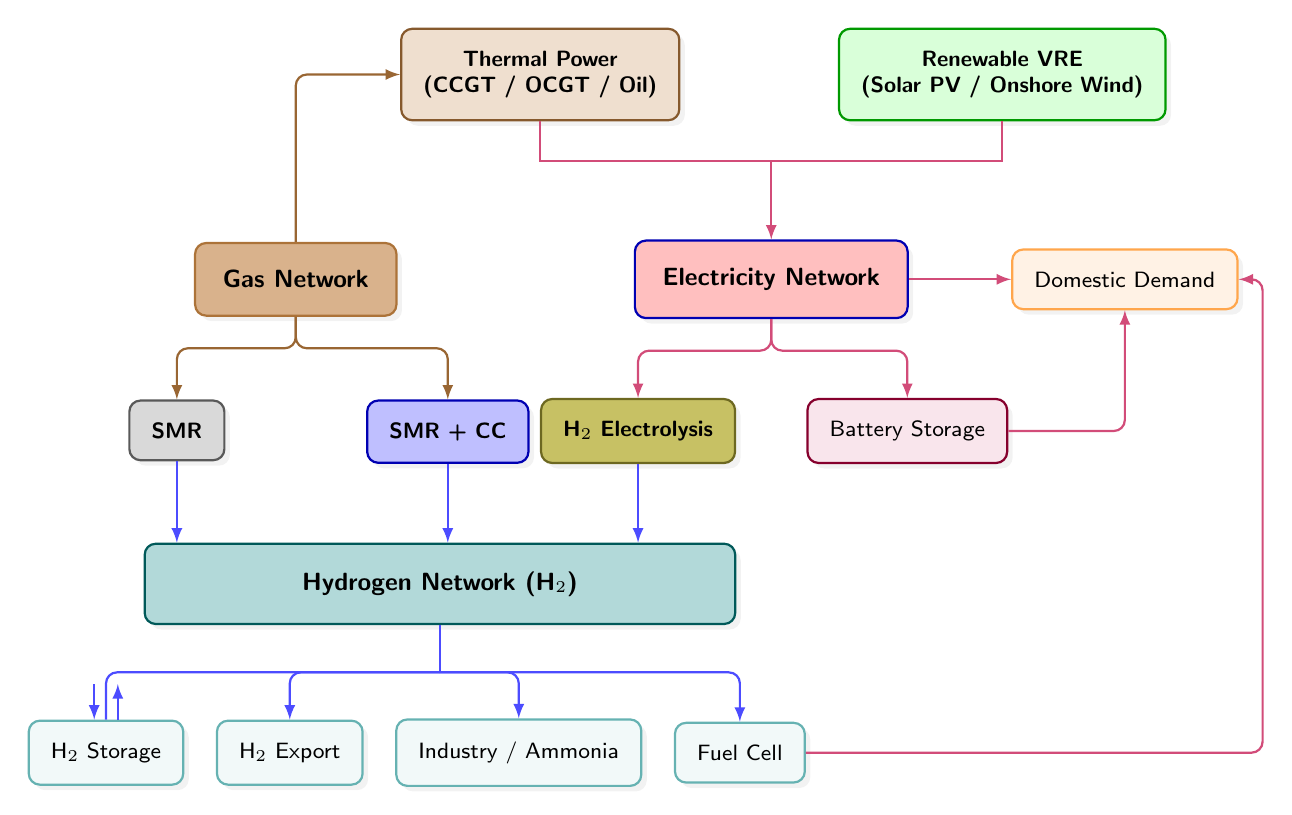
\begin{tikzpicture}[
    % Base node styling
    base/.style={
        draw=gray!60,
        thick,
        rectangle,
        rounded corners=4pt,
        align=center,
        inner sep=8pt,
        font=\sffamily\footnotesize,
        drop shadow={opacity=0.1, shadow xshift=2pt, shadow yshift=-2pt}
    },
    % Sector-specific block stylings
    vreNode/.style={
        base,
        draw=green!60!black,
        fill=green!15,
        font=\sffamily\bfseries\footnotesize
    },
    thermalNode/.style={
        base,
        draw=brown!70!black,
        fill=brown!25,
        font=\sffamily\bfseries\footnotesize
    },
    gasNode/.style={
        base,
        draw=brown!90!black,
        fill=brown!60,
        text=black,
        font=\sffamily\bfseries\small,
        inner sep=10pt
    },
    gridNode/.style={
        base,
        draw=blue!70!black,
        fill=red!25,
        text=black,
        font=\sffamily\bfseries\small,
        inner sep=10pt
    },
    demandNode/.style={
        base,
        draw=orange!70,
        fill=orange!10,
        font=\sffamily\footnotesize
    },
    storageNode/.style={
        base,
        draw=purple!70!black,
        fill=purple!10
    },
    h2ProdNode/.style={
        base,
        draw=olive!70!black,
        fill=olive!50,
        font=\sffamily\bfseries\footnotesize
    },
    h2BusNode/.style={
        base,
        draw=teal!70!black,
        fill=teal!30,
        text=black,
        font=\sffamily\bfseries\small,
        inner sep=10pt
    },
    h2DestNode/.style={
        base,
        draw=teal!60,
        fill=teal!5
    },
    % Connection lines
    connector/.style={
        draw=black!70,
        -latex,
        thick,
        rounded corners=4pt
    },
    connector_h2/.style={
        draw=blue!70,
        -latex,
        thick,
        rounded corners=4pt
    },
    connector_ac/.style={
        draw=purple!70,
        -latex,
        thick,
        rounded corners=4pt
    },
    gasConnector/.style={
        draw=brown!80!black,
        -latex,
        thick,
        rounded corners=4pt
    },
    h2ProdNode2/.style={
        base,
        draw=gray!70!black,
        fill=gray!30,
        font=\sffamily\bfseries\footnotesize
    },
    h2ProdNode3/.style={
        base,
        draw=blue!70!black,
        fill=blue!25,
        font=\sffamily\bfseries\footnotesize
    }
]

    % --- LEVEL 1: GENERATION SOURCE BLOCKS ---
    \node[thermalNode] (thermal) {Thermal Power \\ (CCGT / OCGT / Oil)};
    \node[vreNode, right=2.0cm of thermal] (vre) {Renewable VRE \\ (Solar PV / Onshore Wind)};

    % --- LEVEL 2: INFRASTRUCTURE NETWORKS & DEMAND ---
    \node[gridNode, below=1.5cm of $(thermal.south)!0.5!(vre.south)$] (grid) {Electricity Network};
    \node[gasNode, left=3.0cm of grid] (gasnet) {Gas Network};
    \node[demandNode, right=1.3cm of grid] (demand) {Domestic Demand};

    % --- LEVEL 3: PRODUCTION & STORAGE INTERFACES (Reorganized Horizontally) ---
    % Gas branching components
    \node[h2ProdNode2, below left=1.05cm and -0.4cm of gasnet] (smr) {SMR};
    \node[h2ProdNode3, below right=1.05cm and -0.4cm of gasnet] (smrcc) {SMR + CC};
    
    % Electricity branching components (Exchanged positions)
    \node[h2ProdNode, below left=1cm and -1.3cm of grid] (electrolysis) {H$_2$ Electrolysis};
    \node[storageNode, below right=1cm and -1.3cm of grid] (battery) {Battery Storage};

    % --- LEVEL 4: HYDROGEN CARRIER BUS (Spans across all three production blocks) ---
    \node[h2BusNode, below=1cm of smrcc, xshift=-0.1cm, minimum width=7.5cm] (h2bus) {Hydrogen Network (H$_2$)};

    % --- LEVEL 5: HYDROGEN STORAGE, EXPORT & OFFTAKES ---
    \node[h2DestNode, below right=1.2cm and -9.0cm of h2bus] (cavern) {H$_2$ Storage};
    \node[h2DestNode, right=0.4cm of cavern] (export) {H$_2$ Export};
    \node[h2DestNode, right=0.4cm of export] (ammonia) {Industry / Ammonia};
    \node[h2DestNode, right=0.4cm of ammonia] (fuelcell) {Fuel Cell};


    % --- CONNECTIONS & FLOW ARCHITECTURE ---

    % Gas Network Connections (North to Thermal, South to SMR / SMR+CC)
    \draw[gasConnector] (gasnet.north) |- (thermal.west);
    \draw[gasConnector] (gasnet.south) -- ++(0,-0.4) -| (smr.north);
    \draw[gasConnector] (gasnet.south) -- ++(0,-0.4) -| (smrcc.north);

    % Generation feeds into Grid via horizontal merge
    \coordinate (genMerge) at ($(thermal.south)!0.5!(vre.south) + (0,-0.5)$);
    \draw[thick, purple!70] (thermal.south) -- ++(0,-0.5) -- (vre.south |- genMerge) -- (vre.south);
    \draw[connector_ac] (genMerge) -- (grid.north);

    % Grid out-flow to Direct Demand
    \draw[connector_ac] (grid.east) -- (demand.west);

    % Grid output split to Electrolysis and Battery
    \draw[connector_ac] (grid.south) -- ++(0,-0.4) -| (electrolysis.north);
    \draw[connector_ac] (grid.south) -- ++(0,-0.4) -| (battery.north);

    % Triple Production Core feeding vertically down into the Hydrogen Bus north face
    \draw[connector_h2] (smr.south) -- (smr.south |- h2bus.north);
    \draw[connector_h2] (smrcc.south) -- (smrcc.south |- h2bus.north);
    \draw[connector_h2] (electrolysis.south) -- (electrolysis.south |- h2bus.north);

    % H2 Bus Distribution Fork to Offtakes
    \path (h2bus.south) -- ++(0,-0.6) coordinate (h2fork);
    \draw[thick, blue!70] (h2bus.south) -- (h2fork);
    
    % Main structural line down to Cavern (without an arrow head at the fork)
    \draw[thick, draw=blue!70, rounded corners=4pt] (h2fork) -| (cavern.north);
    
    % Dual localized arrows directly at the Cavern node entrance face
    \draw[latex-, thick, draw=blue!70] ($(cavern.north) + (-0.15cm, 0)$) -- ++(0, 0.45cm);
    \draw[-latex, thick, draw=blue!70] ($(cavern.north) + (0.15cm, 0)$) -- ++(0, 0.45cm);
    
    % Standard unidirectional arrows for the remaining offtakes
    \draw[connector_h2] (h2fork) -| (export.north);
    \draw[connector_h2] (h2fork) -| (ammonia.north);
    \draw[connector_h2] (h2fork) -| (fuelcell.north);

    % Battery feedback loop directly into south-center (left anchor offset)
    \draw[connector, purple!70] (battery.east) -| (demand.south);

    % Fuel Cell feedback loop directly into south-center (right anchor offset)
    \draw[connector, purple!70] (fuelcell.east) -- ++(5.8,0) |- (demand.east);

\end{tikzpicture}
\end{document}
